\documentclass[11pt,compress,t,notes=noshow, aspectratio=169, xcolor=table]{beamer}

\usepackage{../../style/lmu-lecture}
% Defines macros and environments
% This file is included in slides and exercises

% Rarely used fontstyle for R packages, used only in 
% - forests/slides-forests-benchmark.tex
% - exercises/single-exercises/methods_l_1.Rnw
% - slides/cart/attic/slides_extra_trees.Rnw
\newcommand{\pkg}[1]{{\fontseries{b}\selectfont #1}}

% Spacing helpers, used often (mostly in exercises for \dlz)
\newcommand{\lz}{\vspace{0.5cm}} % vertical space (used often in slides)
\newcommand{\dlz}{\vspace{1cm}}  % double vertical space (used often in exercises, never in slides)
\newcommand{\oneliner}[1] % Oneliner for important statements, used e.g. in iml, algods
{\begin{block}{}\begin{center}\begin{Large}#1\end{Large}\end{center}\end{block}}

% Don't know if this is used or needed, remove?
% textcolor that works in mathmode
% https://tex.stackexchange.com/a/261480
% Used e.g. in forests/slides-forests-bagging.tex
% [...] \textcolor{blue}{\tfrac{1}{M}\sum^M_{m} [...]
% \makeatletter
% \renewcommand*{\@textcolor}[3]{%
%   \protect\leavevmode
%   \begingroup
%     \color#1{#2}#3%
%   \endgroup
% }
% \makeatother


\title{Interpretable Machine Learning}
% \author{LMU}
%\institute{\href{https://compstat-lmu.github.io/lecture_iml/}{compstat-lmu.github.io/lecture\_iml}}
\date{}

\begin{document}

\newcommand{\titlefigure}{figure/h-statistic}
\newcommand{\learninggoals}{
\item Understand Friedman's H-statistic
\item Measure 2-way interactions between pairs of features
\item Measure a feature's overall interaction strength
}

\lecturechapter{Friedman's H-Statistic}
\lecture{Interpretable Machine Learning}

\begin{frame}{Idea \citebutton{Friedman and Popescu (2008)}{https://doi.org/10.1214/07-AOAS148}}

    \textbf{2-way interaction:} If two features $j$ and $k$ do not interact, their mean-centered PD function is

	$$\fh_{jk, PD}(x_j, x_k) = \fh_{j, PD}(x_j) + \fh_{k, PD}(x_k)$$

\begin{itemize}
	\item $\fh_{jk, PD}(x_j, x_k)$: joint 2-dim PD function of feature $j$ and $k$
	\item $\fh_{j, PD}(x_j)$ and $\fh_{k, PD}(x_k)$: 1-dim PD functions of single features $j$ and $k$
\end{itemize}

\end{frame}
\begin{frame}{Idea}

	\textbf{Overall interaction:} If feature $j$ does not interact with any other feature (denoted by index $-j$), the mean-centered prediction function can be decomposed by

	$$\fh(\xv) = \fh_{j, PD}(x_j) +  \fh_{-j, PD}(\xv_{-j})$$

\begin{itemize}
	\item $\fh(\xv)$: mean-centered prediction function
	\item $\fh_{j, PD}(x_j)$: 1-dim PD function of feature $j$
	\item $\fh_{-j, PD}(\xv_{-j})$: $(p-1)$-dim PD function of all $p$ features except feature $j$
\end{itemize}
\end{frame}

\begin{frame}{2-way Interaction Strength}
H-statistic measures interaction strength between feature $j$ and $k$ by

	$$H^2_{jk} = \frac{\sum_{i=1}^n\left[\fh_{jk,PD}(x_j^{(i)}, x_k^{(i)}) - \fh_{j, PD}(x_j^{(i)}) - \fh_{k, PD}(x_k^{(i)})  \right]^2}{\sum_{i=1}^n \left[\fh_{jk,PD}(x_j^{(i)}, x_k^{(i)}) \right]^2}$$

\textbf{Note}: The numerator is $0$ if the two features $x_j$ and $x_k$ do not interact, i.e., $\fh_{jk, PD}(x_j, x_k) - \fh_{j, PD}(x_j) - \fh_{k, PD}(x_k) = 0$.

$\Rightarrow$ The smaller the values of $H^2_{jk}$, the weaker the interaction between $x_j$ and $x_k$.


%\footnote[frame]{Friedman, Jerome H., and Bogdan E. Popescu (2008). Predictive learning via rule ensembles. The Annals of Applied Statistics. JSTOR, 916–54.}

\end{frame}


\begin{frame}{Overall Interaction Strength}

Similarly, it is possible to measure whether a feature $j$ interacts with any other feature (Overall interaction strength):


$$H^2_{j} = \frac{\sum_{i=1}^n\left[\fh(x^{(i)}) - \fh_{j, PD}(x_j^{(i)}) - \fh_{-j, PD}(x_{-j}^{(i)})  \right]^2}{\sum_{i=1}^n \left[\fh(x^{(i)}) \right]^2}$$

\textbf{Example}: Inspect interactions of a random forest for the bike data

\begin{center}
	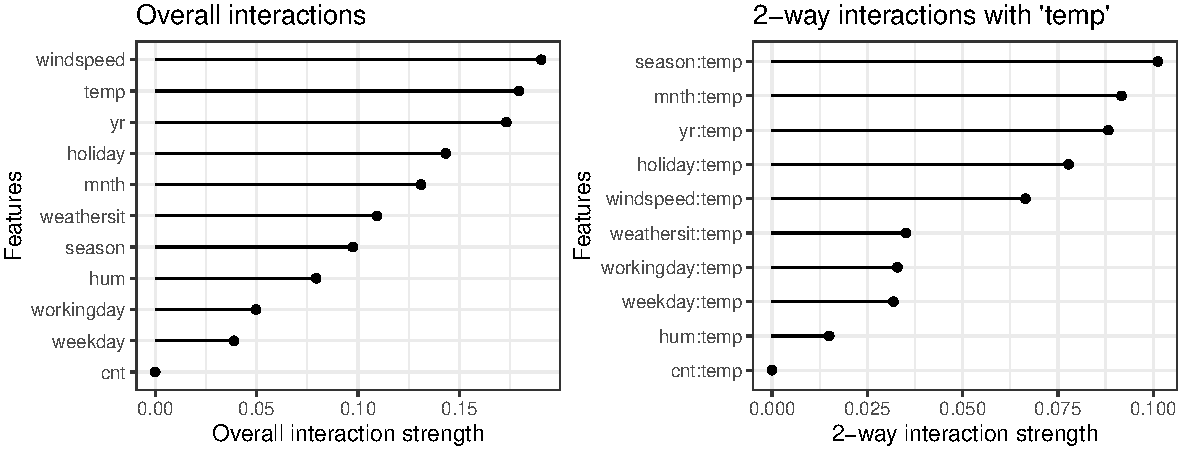
\includegraphics[width=0.7\textwidth]{figure/h-statistic}
\end{center}
\end{frame}


\endlecture
\end{document}
